% !TeX spellcheck = en_EN
% !TeX encoding = UTF-8
% !TeX program = xelatex
%----------------------------------------------------------------------------
\chapter{Modeling and Code Generation}
%----------------------------------------------------------------------------

This chapter covers various aspects related to modeling and code generation. It begins by discussing the difficulties that arise when generating code from low-level model descriptors for embedded systems. The chapter then goes on to cover the Gamma statecharts and its composition language, model transformations, and mapping XSTS to C code.

%----------------------------------------------------------------------------
\section{Code Generation for Embedded Systems}
%----------------------------------------------------------------------------

This section discusses the challenges that arise when generating code from low-level models. Embedded systems software is required to run on various hardware architectures to ensure flexibility and portability on different hardware components, reduce constraints on physical device selection, and provide long term support. Therefore, a high-level design language is needed to model the reactive system's behavior independently of the hardware and to enable software development on multiple platforms. 

UML Statecharts serve best as the high-level design language for modeling component based reactive systems due to their ability to capture complex state behavior and event handling, greatly reducing complexity compared to programmer-made code. Gamma provides a composite language to build compositions of statecharts which helps to reduce complexity and increase modularity. As of now, Gamma lacks the capability to generate platform independent code apart from the already existing Java code generator which is not optimal for embedded systems due to its high resource requirements and lack of real-time support. The following objectives should be met by a code generator intended for embedded systems:

\begin{itemize}
	\item \textbf{Limited resources:} The code should be runnable on wide-range of hardware architectures. Its choice of language should consider resource requirements and compiler support for embedded hardware.
	
	\item \textbf{Portability:} The generated code should be portable across different platforms to allow for flexibility and use among different domains, from the use of embedded Linux to programming microcontrollers.
	
	\item \textbf{Safety and reliability:} Embedded systems are often used in critical applications such as medical devices and transportation systems, therefore the generated code should be safe and reliable.
\end{itemize}

Considering the aforementioned requirements, I have opted for the C programming language as it demands minimal resources and has extensive support from compilers used for embedded hardware along with software verification tools.

%----------------------------------------------------------------------------
\section{Gamma Statecharts}
%----------------------------------------------------------------------------

In Gamma, components are defined using statecharts, which are based on the Unified Modeling Language (UML). Statecharts consist of states that define the state of the component as well as how it reacts to incoming events. Events are responsible for initiating a possible state change and might have parameters linked to it. Events can come from outside the component, or can be produced by internal timers. Actions are executable statements that are executed when a transition occurs, while guards are conditions that must be met for a transition to occur. Timeout events can be associated with states and transitions in statecharts, which trigger after a specified duration of time. Upon entering or exiting a state, entry and exit actions can be executed. These actions have the ability to fire events. UML Statecharts also include hierarchical states, which allow for the composition of multiple states into a higher-level state, and the ability to nest states within other states. Shallow and deep history states store the last active state of a higher-level state when it is exited. When re-entering the high-level state, the active inner state will be the one stored by the history state in case of deep history.

\begin{figure}[h]
	\centering
	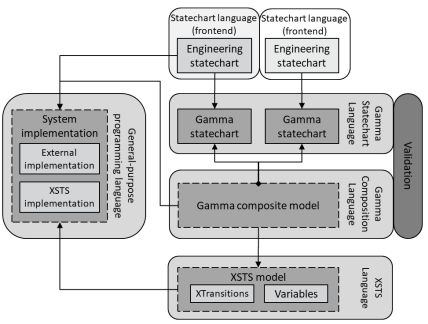
\includegraphics[width=0.6\textwidth]{images/gamma.png}
	\caption{The route of models to code generation.}
	\label{fig:gamma}
\end{figure}

Statecharts provide a high-level representation of a system's logic. While manual implementation of this behavior is possible, it is error-prone and time-consuming. Automatic code generation can eliminate these issues, but it requires a bridge between the high-level statechart model and the low-level programming language. Gamma addresses this issue by transforming its statechart components into low-level representations, which enables developers to work with high level models, such as statecharts, while code generators can utilize the generated low-level representations.

%----------------------------------------------------------------------------
\section{Model Transformation}
%----------------------------------------------------------------------------

Model transformations play a crucial role in the code generation process, enabling the conversion of statechart models through various stages to achieve specific goals. The sequence begins with UML statecharts obtained from Yakindu, a popular modeling tool. These UML statecharts are being transformed into the Gamma statechart language, from which Gamma compositions can be created using the Gamma composite definition language. Gamma compositions allow for the combination of multiple statecharts to create complex systems.

To facilitate formal verification, the Gamma compositions can then be transformed into languages recognized by specific model checkers such as UPPAAL, Theta, or Spin. Another transformation step involves converting the statechart descriptors or compositions into the XSTS language. Although this intermediate step is not discussed in detail here, it serves as a bridge between Gamma languages and XSTS.

\begin{figure}[h]
	\centering
	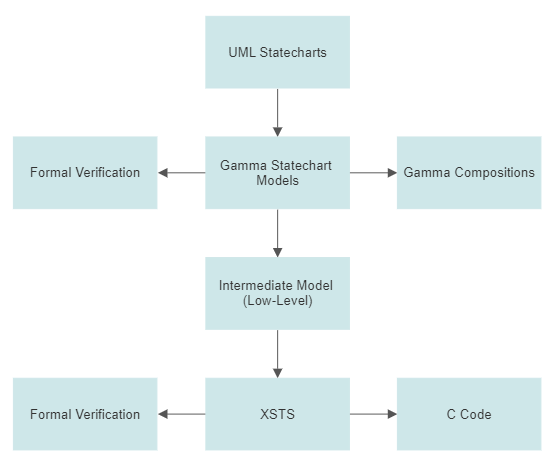
\includegraphics[width=0.8\textwidth]{images/transformation.png}
	\caption{Model transformations using Gamma.}
	\label{fig:transformation}
\end{figure}

The XSTS models serve as the foundation for generating code in languages like C or Java. Moreover, the XSTS models can be utilized for formal verification by further transforming them into languages recognized by the model checkers mentioned earlier. This enables comprehensive formal verification of the system's properties and ensures its correctness and reliability. By acquiring these test cases in the Gamma test language, we can transform them further into test cases to not only verify our model but the code generated by the generator itself.

%----------------------------------------------------------------------------
\section{Mapping XSTS to C Code}
%----------------------------------------------------------------------------

Once a statechart model has been transformed to its low-level descriptor, it needs to be translated to C language to be compiled and executed on the target platform. In the context of this paper, the XSTS model is transformed into C code. This process requires mapping the elements and behavior of the XSTS language onto constructs and syntax within the C language. 

Since the code generator uses a version of XSTS serialized to XML, containing specific types of generated objects by using Eclipse EMF we cannot explicitly map XSTS keywords to C expressions. However the structure of one can be easily corresponded to another. 

The mapping begins with the type definitions present in the XSTS model. These type definitions are mapped to C enums. The enums serve as symbolic representations of the regions and states within the system. Following the type definitions, the variable declarations in the XSTS model are mapped to variables in the C code. These variables represent the underlying mechanism of the component. In the C code, these variables are declared within a struct. Common data types used in the variable declarations include integers (unsigned if the XSTS variable has a ClockVariable annotation), floats, booleans, and the previously mentioned enums.
\bigskip

\begin{lstlisting}[language=C, caption={Representation of regions in XSTS}]
	<typeDeclarations name="Main_region_Controller">
		<type xsi:type="hu.bme.mit.gamma.expression:EnumerationTypeDefinition">
			<literals name="__Inactive__"/>
			<literals name="Operating"/>
			<literals name="Interrupted"/>
		</type>
	</typeDeclarations>
\end{lstlisting}

The XSTS model includes variable groups, specifically SystemInputGroups and SystemOutputGroups, along with their associated ParameterGroups. These groups are mapped to ports in the C code, effectively generating setters and getters for the system's inputs and outputs. Furthermore, the XSTS model contains initializing transitions, which define the initial state and behavior of the system. These transitions are consisting mainly of value definitions, setting initial values for variables within the struct.

Finally, the XSTS model includes transitions that consist of actions and expressions. These transitions capture the core logic and behavior of the system. Actions and expressions are mapped to their respective counterparts in the C code. Due to the extensive number of actions and expressions present in the XSTS model, it is impractical to individually introduce each one within the scope of this section.

